\documentclass[11pt]{amsart}
\usepackage{geometry}                % See geometry.pdf to learn the layout options. There are lots.
\geometry{letterpaper}                   % ... or a4paper or a5paper or ... 
%\geometry{landscape}                % Activate for for rotated page geometry
%\usepackage[parfill]{parskip}    % Activate to begin paragraphs with an empty line rather than an indent
\usepackage{graphicx}
\usepackage{amssymb}
\usepackage{epstopdf}
\usepackage[usenames,dvipsnames]{color}
\usepackage{fancyvrb}
\usepackage{listings}
\usepackage{booktabs,footmisc}
\usepackage{hyperref}
\usepackage[all]{hypcap}

\usepackage{topcapt}


 
% include the lines below to use a nicer fixed-width font than the default one
 
\lstset{fancyvrb=true}
\lstset{
	basicstyle=\small\tt,
	identifierstyle=,
	commentstyle=\color{Bittersweet},
	stringstyle=\color{red},
	showstringspaces=false,
	tabsize=3,
	numbers=left,
	captionpos=b,
	xleftmargin=2em
%	numberstyle=\tiny
	%stepnumber=4
	}
\DeclareGraphicsRule{.tif}{png}{.png}{`convert #1 `dirname #1`/`basename #1 .tif`.png}

\title{ReLogo Getting Started Guide}
\author{Jonathan Ozik - Repast Development Team}
\date{\today}                                           % Activate to display a given date or no date

\begin{document} 
\maketitle
\setcounter{section}{-1}

\section{Before we Get Started}
Before we can do anything with ReLogo, we need to make sure that we have a proper installation of Repast Simphony 2.0. Instructions on downloading and installing Repast Simphony on various platforms can be found on the \href{http://repast.sourceforge.net/download.html}{Repast website}.

\section{Getting Started with ReLogo}
Now let us begin our exploration of ReLogo. We will be building a simple agent-based model involving  zombies chasing humans and humans running away from zombies. Our approach will be to not overwhelm you but to explain only as much as is needed at each step. By the end of this chapter, we'll have covered a lot of ground and you'll be able to continue with your own explorations of ReLogo.

The first thing we must do is create a new ReLogo project. This is done by clicking on the New ReLogo Project icon in the toolbar (Fig.~\ref{fig:newprojecticon}) at the top of our ReLogo workspace\footnote{The default workspace that came with your Repast Simphony installation should be set up correctly. However, if you have modified the settings or are using a custom workspace see Section~\ref{sec:defworkspace} for the preferred ReLogo workspace settings.}.

\begin{figure}[h]
\begin{center}
\vspace{.2in}
\centerline {
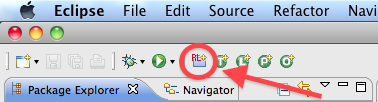
\includegraphics[width=3in]{GettingStartedImages/NewProject.png}
}
\caption{The New ReLogo Project icon.}
\label{fig:newprojecticon}
\end{center}
\end{figure}

This brings up the New ReLogo Project Wizard (Fig.~\ref{fig:newprojectwiz}) which gives us the ability to name our project (and a few more options which we'll ignore for now). Typing in ``Zombies" in the ``Project name" field\footnote{ReLogo differentiates between capitalized and uncapitalized letters (i.e., it is case sensitive) so, when following this tutorial, it will be important to note the capitalization of names, variables, etc.}, we press the ``Finish" button and the wizard sets up our project. The project structure should look like Fig.~\ref{fig:projectstructure} (but if it does not, see this note\footnote{Here we assume that your ReLogo Resource Filter is enabled. If the ReLogo Resource Filter is disabled, you may see more elements in your Zombies project. See Section~\ref{sec:RRF} on how to disable/enable this filter.}).

\begin{figure}[h]
\begin{center}
\vspace{.2in}
\centerline {
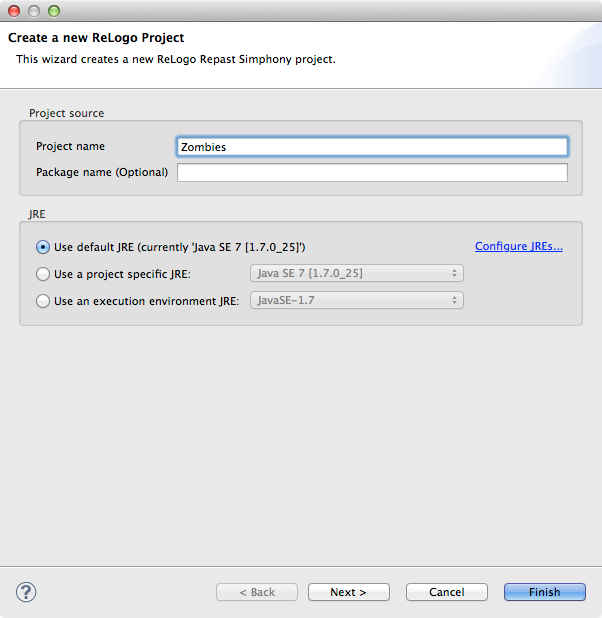
\includegraphics[width=3in]{GettingStartedImages/NewProject2.png}
}
\caption{The New ReLogo Project Wizard.}
\label{fig:newprojectwiz}
\end{center}
\end{figure}

\begin{figure}[h]
\begin{center}
\vspace{.2in}
\centerline {
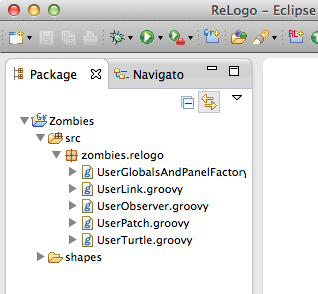
\includegraphics[width=3in]{GettingStartedImages/ZombiesDirectoryStructure.png}
}
\caption{The directory structure of the newly created Zombies project.}
\label{fig:projectstructure}
\end{center}
\end{figure}

What we see is the Zombies project folder, the ``src" subfolder, the ``zombies.relogo" package, and the relevant ReLogo files, in addition to a ``shapes" folder. More on each of these things as we proceed.

\subsection{Creating the Human and Zombie turtle types}

Now that we have all our model infrastructure in place, we can start specifying the details of our Zombie model. First, since zombies love to chase humans, we create the Human turtle\footnote{In Logo dialects a ``turtle" is a mobile agent.} type\footnote{Many of the ReLogo entities we'll encounter, including turtle types,  are what are known in Object Oriented programming languages as \emph{classes}.}. We do this by selecting the ``zombies.relogo" package, if it isn't selected, and then clicking on the New Turtle icon (Fig.~\ref{fig:newturtleicon}) in the toolbar\footnote{Selecting the ``zombies.relogo" package simplifies the next step.}. This brings up the New Turtle Wizard (Fig.~\ref{fig:humanwizard}) which allows us to specify the name of our turtle type (Human). If we initially selected the ``zombies.relogo" package, we simply fill in the Name field with ``Human" and hit the Finish button\footnote{If the ``zombies.relogo" package hadn't been selected, we need to fill in the Package field with ``zombies.relogo" before hitting the Finish button.}. At this point we should be greeted by our newly created Human turtle type as seen in Fig.~\ref{fig:humantype}\footnote{For those curious about the .groovy file ending, ReLogo is an agent-based modeling domain specific language (ABM DSL), written in the  \href{http://groovy.codehaus.org/}{Groovy} programming language. While it isn't necessary to be able to follow this getting started guide, we recommend getting to know the language through the Groovy website and the many Groovy books which are available. There is also a very convenient \href{http://groovyconsole.appspot.com/}{web based console} where you can experiment with Groovy.}

\begin{figure}
\begin{center}
\vspace{.2in}
\centerline {
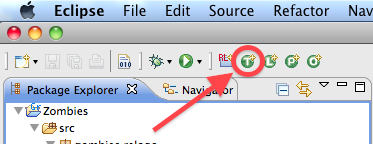
\includegraphics[width=3in]{GettingStartedImages/NewTurtle.png}
}
\caption{The New Turtle icon.}
\label{fig:newturtleicon}
\end{center}
\end{figure}

\begin{figure}
\begin{center}
\vspace{.2in}
\centerline {
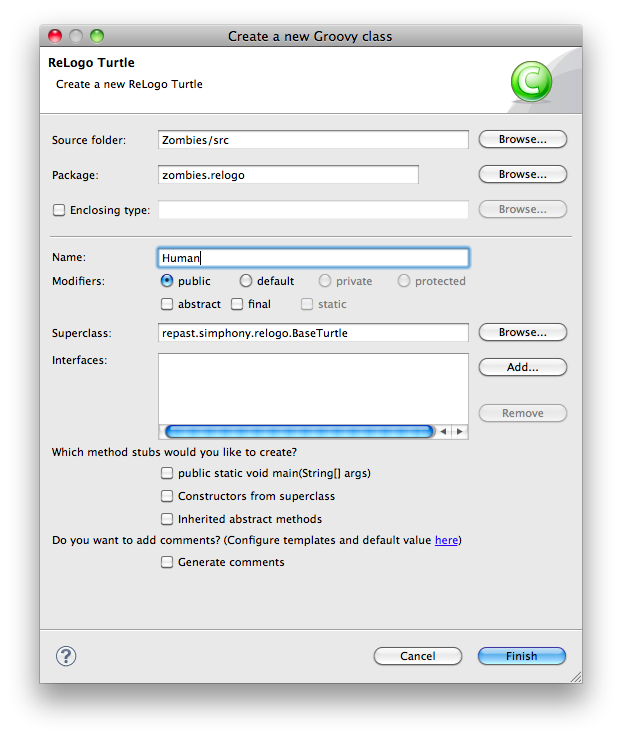
\includegraphics[width=3in]{GettingStartedImages/Human1.png}
}
\caption{The New Turtle Wizard with information for creating the Human turtle type.}
\label{fig:humanwizard}
\end{center}
\end{figure}

\begin{figure}
\begin{center}
\vspace{.2in}
\centerline {
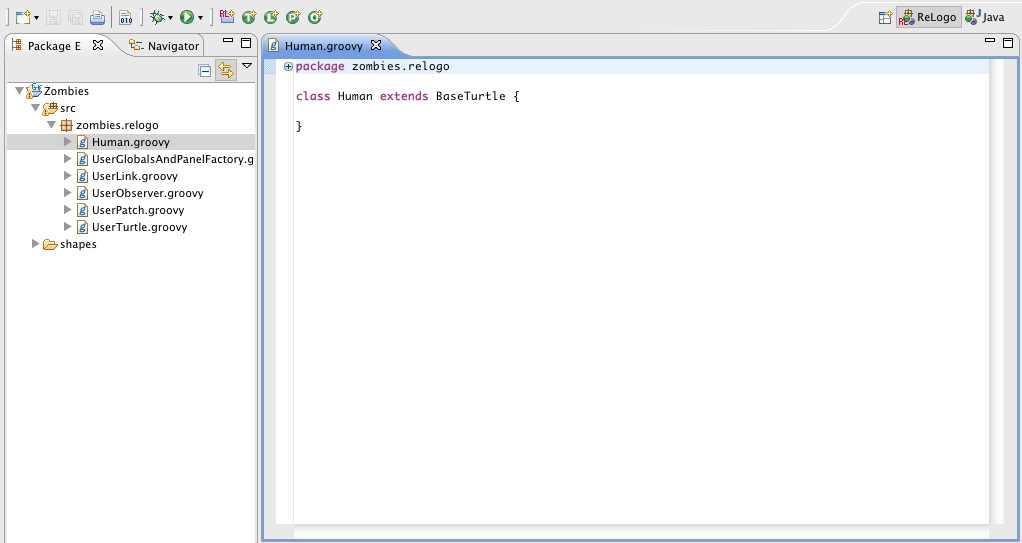
\includegraphics[width=4in]{GettingStartedImages/Human2.png}
}
\caption{The view after creation of the Human turtle type.}
\label{fig:humantype}
\end{center}
\end{figure}

Next we follow a similar procedure to create the Zombie turtle type (Fig.~\ref{fig:zombiewizard}).

\begin{figure}
\begin{center}
\vspace{.2in}
\centerline {
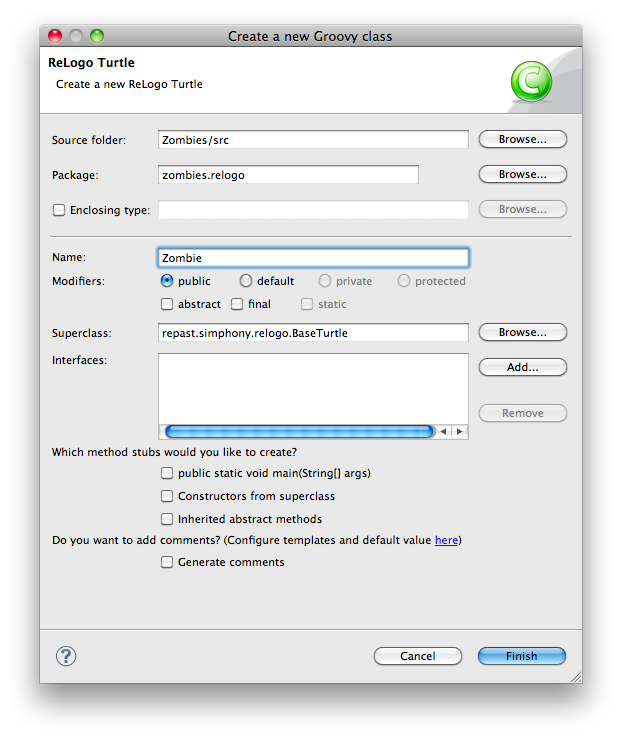
\includegraphics[width=3in]{GettingStartedImages/Zombie1.png}
}
\caption{The New Turtle Wizard with information for creating the Zombie turtle type.}
\label{fig:zombiewizard}
\end{center}
\end{figure}

\clearpage
\subsection{Defining Human and Zombie behaviors.}
The next step in building our model is defining the behaviors of the Human and Zombie turtle types. We'll dive right in. 

Each Human will have a \emph{step} method which looks like this (but first, see important note\footnote{For those following this getting started guide electronically, simple copying-and-pasting of the code from the tutorial will result in errors. Even if the line numbers are removed there can be errors resulting from the formatting of quoted strings and other elements. In short, to get the most out of the guide with the least amount of errors, we recommend typing in the code yourself.}):

\noindent\begin{minipage}[h]{\textwidth}
\vspace{.2in}
\lstset{language=java,caption=Human step method.,label=lst:humanstep}
\begin{lstlisting}
def step(){
	def winner = minOneOf(neighbors()){
		count(zombiesOn(it))
	}
	face(winner)
	forward(1.5)
	if (infected){
		infectionTime++
		if (infectionTime >= 5){
			hatchZombies(1){
				size = 2
			}
			die()
		}
	}
}
\end{lstlisting}
\vspace{.2in}
\end{minipage}

The thinking here is that at every time advancement of our simulation, or ``tick,'' each Human will execute this method. The Human first chooses a \emph{winner} which is, in plain English, one of the neighboring patches\footnote{Patches were introduced by \href{http://education.mit.edu/starlogo/}{StarLogo} and are square shaped immobile agents which make up an underlying grid structure in a ReLogo world.} with the fewest number of Zombies on it. When the winner is chosen, the Human \emph{face}s it and moves \emph{forward} 1.5 steps, thereby running away from potential high Zombie areas. If the Human is \emph{infected}, and 5 or more time ticks have passed since the initial infection, the Human \emph{die}s and \emph{hatch}es a Zombie.

Let's briefly review the code. A ReLogo turtle has a number of ReLogo primitives\footnote{The set of available primitives can be found in the ReLogoPrimitives.html file that came with the Repast Simphony distribution. The primitives are separated broadly by the type of ReLogo entity that uses them and further by the type of primitive category (e.g, motion, rotation, etc.). Clicking on a primitive will give you more details. This will likely be your primary reference as you explore ReLogo so it will help to get familiar with it. }, or capabilities, it can use, without having to create its own. Among these are \emph{minOneOf} and \emph{neighbors}. \emph{minOneOf} takes as an argument a set of ``things" and a block defining what quantity will be used to determine the minimum of.

The ``things'' (in line 2 of Listing~\ref{lst:humanstep}) are the set of patches returned by the \emph{neighbors} primitive, which are the 8 neighbors\footnote{This is referred to as the Moore neighborhood in a grid.} of the patch that the Human is on. You'll notice that \emph{neighbors} is followed by a set of empty parentheses. This is because the primitives are what are referred to in some programming circles as \emph{methods} and the parentheses hold the arguments to those \emph{methods}. If the method doesn't take any arguments, as is the case with the \emph{neighbors} primitive, we still need to call the method but without any arguments. As mentioned above, \emph{minOneOf} takes two arguments, the second being a block of code, specified between curly braces. Groovy allows, for clarity, to omit the parentheses around a block of code if it's the last argument to a method. So instead of writing:

\noindent\begin{minipage}[h]{\textwidth}
\vspace{.2in}
\lstset{language=java, numbers=none}
\begin{lstlisting}
maxOneOf(neighbors() , {
	count(zombiesOn(it))
} )
\end{lstlisting}
\vspace{.2in}
we can write:
\vspace{.2in}
\lstset{language=java}
\begin{lstlisting}
maxOneOf(neighbors()){
	count(zombiesOn(it))
} 
\end{lstlisting}
\vspace{.2in}
\end{minipage}

When you define a turtle type in ReLogo, there are primitives that are automatically made available to various ReLogo entities\footnote{For a complete list, see Table~\ref{tab:zombiemethods} in Appendix~\ref{app:genprims}.}. \emph{zombiesOn} is such a primitive that was made available to turtles when we defined the Zombie turtle type. It takes as an argument a patch\footnote{\emph{zombiesOn} can also take a turtle as an argument, which has the same semantics as the version that takes a patch as an argument, but in the former case the patch is the patch under the turtle.} and returns the Zombie turtles on that patch. The \emph{it} is another feature of Groovy. It is an implicit argument to the block of code\footnote{Arguments passed to a block of code are a comma separated sequence of variable names followed by \texttt{->}. For any block of code without input arguments explicitly specified, the assumption is that it takes one implicit parameter named \emph{it}.} which allows us to simplify:

\noindent\begin{minipage}[h]{\textwidth}
\vspace{.2in}
\lstset{language=java, numbers=none}
\begin{lstlisting}
maxOneOf(neighbors()){ p ->
	count(zombiesOn(p))
} 
\end{lstlisting}
\vspace{.2in}
to:
\vspace{.2in}
\lstset{language=java}
\begin{lstlisting}
maxOneOf(neighbors()){
	count(zombiesOn(it))
} 
\end{lstlisting}
\vspace{.2in}
\end{minipage}

The primitive \emph{count} can be applied to any set of items and returns the number of items in the set. Finally, the \emph{def} keyword in Groovy is used when we define variables or the return types of methods. It's basically a wildcard indicating that whatever it adorns is of ``some" type, without specifying further\footnote{Groovy, for those interested, uses dynamic (but strict) typing. This is just one of the reasons why we often refer to it as a ``less neurotic" Java.}. Thus, taken together, lines 2-4 of Listing~\ref{lst:humanstep}, \emph{assign} to the variable \emph{winner} the patch with the fewest number of Zombies on it\footnote{One of the most common mistakes is replacing the equality operator \texttt{==} with the assignment operator \texttt{=}. In the former case, the \emph{equality} of the two sides is checked and either a \emph{true} or \emph{false} is returned. In the latter case, the right hand side is \emph{assigned} to the left hand side.}.

We'll assume that lines 5 and 6 of Listing~\ref{lst:humanstep} are self explanatory, and proceed to the \emph{conditional} statement on lines 7-13. The \emph{if} keyword is commonly used in many programming languages to determine the logical flow of some statements. In this case, we are checking to see if the Human is \emph{infected} and if so, we proceed to line 8 and otherwise we skip down past line 13, the end of the \emph{if} block. This is a good time to introduce the fact that in addition to methods, ReLogo entities have properties as well. Thus, elsewhere (which we'll show in Listing~\ref{lst:humantype}), we've explicitly specified that the Human turtle type has an \emph{infected} property which we will initially set to \emph{false}. The same holds for the \emph{infectionTime} property\footnote{The \texttt{infectionTime++} notation is a shortcut for \texttt{infectionTime = infectionTime + 1}.}, on line 8, which we'll initially set to 0, again elsewhere (Listing~\ref{lst:humantype}).

On lines 9-12, we check to see if the \emph{infectionTime} is greater than or equal to 5 and, if so, the Human \emph{hatches} a Zombie and then it \emph{dies}\footnote{The order might be confusing but if the Human dies and is removed from the simulation before hatching the Zombie, well, it can't hatch the Zombie!}.

Now let's see what our full Human turtle type looks like, with the \emph{step} method and the turtle properties:

\noindent\begin{minipage}[h]{\textwidth}
\vspace{.2in}
\lstset{language=java,caption=The Human turtle type.,label=lst:humantype}
\begin{lstlisting}
// package declaration and imports, which we can ignore for now

class Human extends BaseTurtle {
	
	def infected = false
	def infectionTime = 0
	
	def step(){
		def winner = minOneOf(neighbors()){
			count(zombiesOn(it))
		}
		face(winner)
		forward(1.5)
		
		if (infected){
			infectionTime++
			if (infectionTime >= 5){
				hatchZombies(1){
					size = 2
				}
				die()
			}
		}
	}
	
}
\end{lstlisting}
\vspace{.2in}
\end{minipage}

The takeaway here is that turtle type properties and methods are defined within the \emph{class} body of the turtle type, in this case between the curly braces on lines 3 and 26.

Now let's move on to the Zombie turtle type. It looks like this:

\noindent\begin{minipage}[h]{\textwidth}
\vspace{.2in}
\lstset{language=java,caption=The Zombie turtle type.,label=lst:zombietype}
\begin{lstlisting}
// package declaration and imports, which we can ignore for now

class Zombie extends BaseTurtle {

	def step(){
		def winner = maxOneOf(neighbors()){
			count(humansOn(it))
		}
		
		face(winner)
		forward(0.5)
		
		if (count(humansHere()) > 0){
			label = "Brains!"
			infect(oneOf(humansHere()))
		}
		else {
			label = ""
		}
	}
	
	def infect(human){
		human.infected = true
	}
}
\end{lstlisting}
\vspace{.2in}
\end{minipage}

What should be noticed here is that, in addition to the method \emph{step}, we've defined another auxiliary method \emph{infect} which takes one argument. Let us take a moment to explore how it's used. Looking at lines 13-15 in Listing~\ref{lst:zombietype}, we see that we check using the primitives \emph{count} and \emph{humansHere}\footnote{As you probably guessed, this is one of the generated primitives when we defined the Human turtle type.} if there are any Human turtle types ``here." If there are, we define the default turtle type property \emph{label} to be ``Brains!" and proceed to \emph{infect} \emph{oneOf} the \emph{humansHere}\footnote{As you likely notice, the purpose of Logo constructs in general and ReLogo code in particular can often easily be understood and can lead to more manageable code.}. To infect the human, we access the human's property \emph{infected} by \emph{referencing} it with a period\footnote{In Object Oriented languages, accessing an object's properties and methods is a common idiom.}.

\subsection{Coordinating behaviors with the UserObserver.}
At this point we have both the Human and Zombie turtle types specified. What we need next is to define the overall flow of our model. Logo uses the notion of an ``observer" to accomplish this role. The UserObserver is the default observer type that was made for us when we created the Zombies project. Double clicking the UserObserver.groovy file in the Package Explorer view (Fig.~\ref{fig:UserObserver}) will bring up the file.

\begin{figure}
\begin{center}
\vspace{.2in}
\centerline {
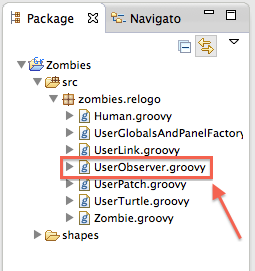
\includegraphics[width=3in]{GettingStartedImages/UserObserver.png}
}
\caption{The UserObserver.groovy file in the Package Explorer view.}
\label{fig:UserObserver}
\end{center}
\end{figure}

A common idiom is to define a method that sets up our simulation. We do so by defining the \emph{setup} method:

\noindent\begin{minipage}[h]{\textwidth}
\vspace{.2in}
\lstset{language=java,caption=The UserObserver setup method.,label=lst:observersetup}
\begin{lstlisting}
def setup(){
	clearAll()
	setDefaultShape(Human, "person")
	createHumans(numHumans){
		setxy(randomXcor(),randomYcor())
	}
	setDefaultShape(Zombie, "zombie")
	createZombies(numZombies){
		setxy(randomXcor(),randomYcor())
		size = 2
	}
}
\end{lstlisting}
\vspace{.2in}
\end{minipage}

We'll first describe, in plain English, what this piece of code does. It is a good idea in any initialization code to reset the simulation, so we first \emph{clearAll} existing entities from the world. Then we define the default shapes of both the Humans and Zombies and create a different number of each (with primitives generated by defining the Human and Zombie turtle types). We also scatter the created turtles randomly across our world and set the size of the Zombies to 2, to make them more prominent.

Now that we know the gist of Listing~\ref{lst:observersetup}, let's delve a little deeper. The \emph{clearAll} primitive removes all existing entities from the ReLogo world and resets the patches to their default state. The \emph{setDefaultShape} primitive takes two arguments. The first argument is a turtle type and the second is a \emph{string}\footnote{A string is a set of characters enclosed in quotes.} specifying a turtle shape. To understand what shapes are available we can open the ``shapes'' folder in the Package Explorer view (Fig.~\ref{fig:shapes}) and see the default shapes that come with any newly created ReLogo project\footnote{In Appendix~\ref{app:drawing} we'll see that you can import a variety of shape types and even create your own.}. Simply specifying the name of one of these shapes (without the .svg suffix) in the \emph{setDefaultShape} primitive's second argument will set the chosen turtle types default shape to it\footnote{This just sets the default shape of the turtle type. Shapes can be subsequently changed during the simulation as well with the shape = ``shapeName'' construct.}.

\begin{figure}
\begin{center}
\vspace{.2in}
\centerline {
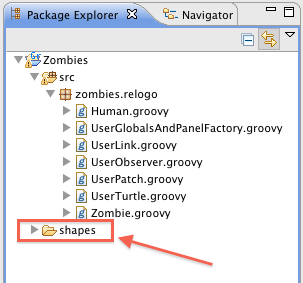
\includegraphics[width=3in]{GettingStartedImages/Shapes.png}
}
\caption{The shapes folder in the Package Explorer view.}
\label{fig:shapes}
\end{center}
\end{figure}


Another thing that the astute reader might notice is that there are references to \emph{numHumans} and \emph{numZombies}. While it's possible for these to be properties of the UserObserver class, we will opt to make these ``tweakable'' as the simulation progresses via slider graphical elements. More on this in a bit. In the meantime we note that the \emph{createTurtleTypes} methods take an optional block of code as a second argument where the created turtles can be initialized immediately after being created.

The next thing for us to do is to define the simulation step. That is, to coordinate what happens with the Zombie and Human turtles as time advances. We do this in our \emph{go} method.

\noindent\begin{minipage}[h]{\textwidth}
\vspace{.2in}
\lstset{language=java,caption=The UserObserver go method.,label=lst:observergo}
\begin{lstlisting}
def go(){
	ask (zombies()){
		step()
	}
	ask (humans()){
		step()
	}
}
\end{lstlisting}
\vspace{.2in}
\end{minipage}
As we see, we've already done most of the hard work of specifying the agents' behaviors. What the observer does is \emph{ask} the Zombie and Human turtle types to execute their \emph{step}. This is achieved with the Logo idiom \emph{ask}. A ReLogo entity (observer, turtle, patch, etc.) can \emph{ask} another entity or set of entities to do things by specifying the request in a block of code after the \emph{ask} primitive\footnote{The block of code is the second argument to the \emph{ask} primitive.}. In this case, the \emph{zombies} and \emph{humans} primitives\footnote{Some more examples of automatically generated primitives.} return the set of all Zombie and Human turtle types respectively. What we notice in the code block passed to \emph{ask} is that we don't need to specify whose \emph{step} method should be run. It's automatically understood to be in the context of the \emph{ask}ed entities.

Collecting what we've covered so far in the observer code, the UserObserver class should look like this\footnote{A clarifying note on comments in program code. Comments in ReLogo and Groovy (and Java) are specified by \texttt{//} for single line comments and \texttt{/*comment content*/} for multiline comments. All the contents of comments are ignored in terms of program logic but they are helpful (and many say indispensable) for creating readable and manageable code.}:

\noindent\begin{minipage}[h]{\textwidth}
\vspace{.2in}
\lstset{language=java,caption=The UserObserver class.,label=lst:observer}
\begin{lstlisting}
// package declaration and imports, which we can ignore for now

class UserObserver extends BaseObserver{

	/**
	 * Some comments here.
	 */
	
	def setup(){
		clearAll()
		setDefaultShape(Human, "person")
		createHumans(numHumans){
			setxy(randomXcor(),randomYcor())
		}
		setDefaultShape(Zombie, "zombie")
		createZombies(numZombies){
			setxy(randomXcor(),randomYcor())
			size = 2
		}
		
	}
	
	def go(){
		ask (zombies()){
			step()
		}
		ask (humans()){
			step()
		}
	}
	
}
\end{lstlisting}
\vspace{.2in}
\end{minipage}

\subsection{Creating the graphical control and display elements.}
We've specified the agent (turtle) behaviors and the overall flow of our Zombies model. Here we add some controls via graphical elements. The relevant file is UserGlobalsAndPanelFactory.groovy (Fig.~\ref{fig:ugapf}).

\begin{figure}
\begin{center}
\vspace{.2in}
\centerline {
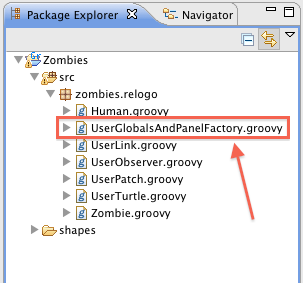
\includegraphics[width=3in]{GettingStartedImages/UserGlobalsAndPanelFactory.png}
}
\caption{The UserGlobalsAndPanelFactory.groovy file in the Package Explorer view.}
\label{fig:ugapf}
\end{center}
\end{figure}

Opening this file we immediately notice some, hopefully helpful, comments on what types of elements are available. For a complete list, see Appendix~\ref{app:graphical}. We'll choose a regular button with a label\footnote{A trailing \texttt{WL}, i.e. ``with label", is added to the graphical element methods to signify that the method takes a label as an argument. Otherwise the name of the relevant object (in the case of a button, the method referred to by the button) will be displayed.} for our \emph{setup} and \emph{go} methods. Regular buttons immediately pop back up when pressed.  We'll choose a toggle button with a label for our \emph{go} method. Toggle buttons remain pressed down when pressed until they're unpressed. They are used to execute methods repeatedly. 

\noindent\begin{minipage}[h]{\textwidth}
\vspace{.2in}
\lstset{language=java, numbers=none}
\begin{lstlisting}
addButtonWL("setup","Setup")
addButtonWL("go","Go Once")
addToggleButtonWL("go","Go")
\end{lstlisting}
\vspace{.2in}
\end{minipage}

We also want to create slider elements, with labels, for the \emph{numHumans} and \emph{numZombies} variables referenced in UserObserver (Listing~\ref{lst:observer}). Sliders allow one to vary the value of a variable by dragging.

\noindent\begin{minipage}[h]{\textwidth}
\vspace{.2in}
\lstset{language=java, numbers=none}
\begin{lstlisting}
addSliderWL("numHumans", "Number of Humans", 1, 1, 100, 50)
addSliderWL("numZombies", "Number of Zombies", 1, 1, 10, 5)
\end{lstlisting}
\vspace{.2in}
\end{minipage}

Let's anticipate that we'd like to know, at any given time, the number of remaining Humans. We employ a monitor for this.

\noindent\begin{minipage}[h]{\textwidth}
\vspace{.2in}
\lstset{language=java, numbers=none}
\begin{lstlisting}
addMonitorWL("remainingHumans", "Remaining Humans", 5)
\end{lstlisting}
\vspace{.2in}
\end{minipage}

A monitor takes as its first argument the name (as a string) of a method in our UserObserver, which we'll have to create below. The second argument is the label of the monitor and the third argument specifies how often we'll be updating the monitor, in this case every 5 time ticks.

Our UserGlobalsAndPanelFactory should look like\footnote{Note that all the graphical elements are specified \emph{within} the curly braces after \emph{addGlobalsAndPanelComponents()}, in this case on lines 7 - 17.}:

\noindent\begin{minipage}[h]{\textwidth}
\vspace{.2in}
\lstset{language=java,caption=The UserGlobalsAndPanelFactory class.,label=lst:ugpf}
\begin{lstlisting}
// package declaration and imports, which we can ignore for now

public class UserGlobalsAndPanelFactory
extends AbstractReLogoGlobalsAndPanelFactory{

	public void addGlobalsAndPanelComponents(){
		
		/**
		 * Example comments
		 */
		
		addButtonWL("setup","Setup")
		addButtonWL("go","Go Once")
		addToggleButtonWL("go","Go")
		addSliderWL("numHumans", "Number of Humans", 1, 1, 100, 50)
		addSliderWL("numZombies", "Number of Zombies", 1, 1, 10, 5)
		addMonitorWL("remainingHumans", "Remaining Humans", 5)
	}
	
}
\end{lstlisting}
\vspace{.2in}
\end{minipage}



The \emph{remainingHumans} method to be added to the UserObserver class is as follows \footnote{As a note, in Groovy the use of the \texttt{return} keyword to return a value from a method is optional when the returned value is given by the last statement in the method. This is because the value of the last statement in a method is automatically returned to the method's caller. Thus we can write \texttt{count(humans())} instead of \texttt{return count(humans())} in Listing~\ref{lst:remainingHumans}.}:

\noindent\begin{minipage}[h]{\textwidth}
\vspace{.2in}
\lstset{language=java, caption=The \emph{remainingHumans} method in UserObserver., label=lst:remainingHumans}
\begin{lstlisting}
def remainingHumans(){
	count(humans())
}
\end{lstlisting}
\vspace{.2in}
\end{minipage}

The UserObserver with the additional \emph{remainingHumans} method should now look like this:

\noindent\begin{minipage}[h]{\textwidth}
\vspace{.2in}
\lstset{language=java,caption=The UserObserver class.,label=lst:observer2}
\begin{lstlisting}
// package declaration and imports, which we can ignore for now

class UserObserver extends BaseObserver{

	/**
	 * Some comments here.
	 */
	
	def setup(){
		clearAll()
		setDefaultShape(Human, "person")
		createHumans(numHumans){
			setxy(randomXcor(),randomYcor())
		}
		setDefaultShape(Zombie, "zombie")
		createZombies(numZombies){
			setxy(randomXcor(),randomYcor())
			size = 2
		}
		
	}
	
	def go(){
		ask (zombies()){
			step()
		}
		ask (humans()){
			step()
		}
	}
	
	def remainingHumans(){
		count(humans())
	}

	
}
\end{lstlisting}
\vspace{.2in}
\end{minipage}

\subsection{Running the Zombies model.}
Our next step is to see what happens when we actually run the Zombies model that we've built so far. We do this by clicking on the small downward triangle to the right of the green ``play" button in the toolbar at the top of the ReLogo workspace (Fig.~\ref{fig:runbutton}). This reveals a pull down menu and we select the ``Zombies Model" choice (Fig.~\ref{fig:runzombies}).

\begin{figure}
\begin{center}
\vspace{.2in}
\centerline {
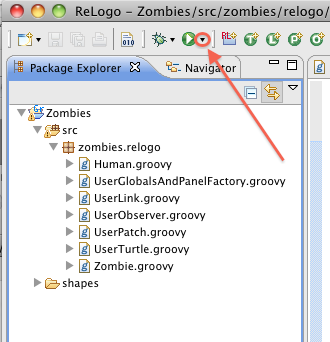
\includegraphics[width=3in]{GettingStartedImages/RunButton.png}
}
\caption{The downward triangle to reveal the Run options pull down menu.}
\label{fig:runbutton}
\end{center}
\end{figure}

\begin{figure}
\begin{center}
\vspace{.2in}
\centerline {
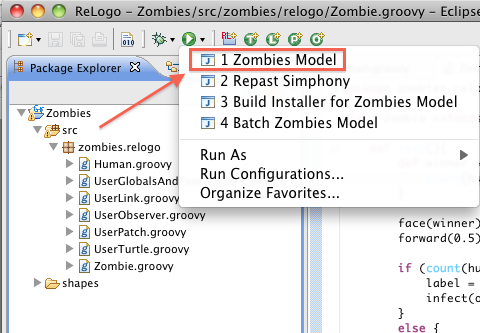
\includegraphics[width=3in]{GettingStartedImages/RunZombies.png}
}
\caption{The ``Zombies Model" entry which launches the Zombies model.}
\label{fig:runzombies}
\end{center}
\end{figure}

This launches the Repast Simphony runtime (Fig.~\ref{fig:repastruntime}). The next step is to press the ``Initialize" button to initialize the runtime (Fig.~\ref{fig:initruntime}) which loads our Zombie model (Fig.~\ref{fig:loadedzombies}).


\begin{figure}
\begin{center}
\vspace{.2in}
\centerline {
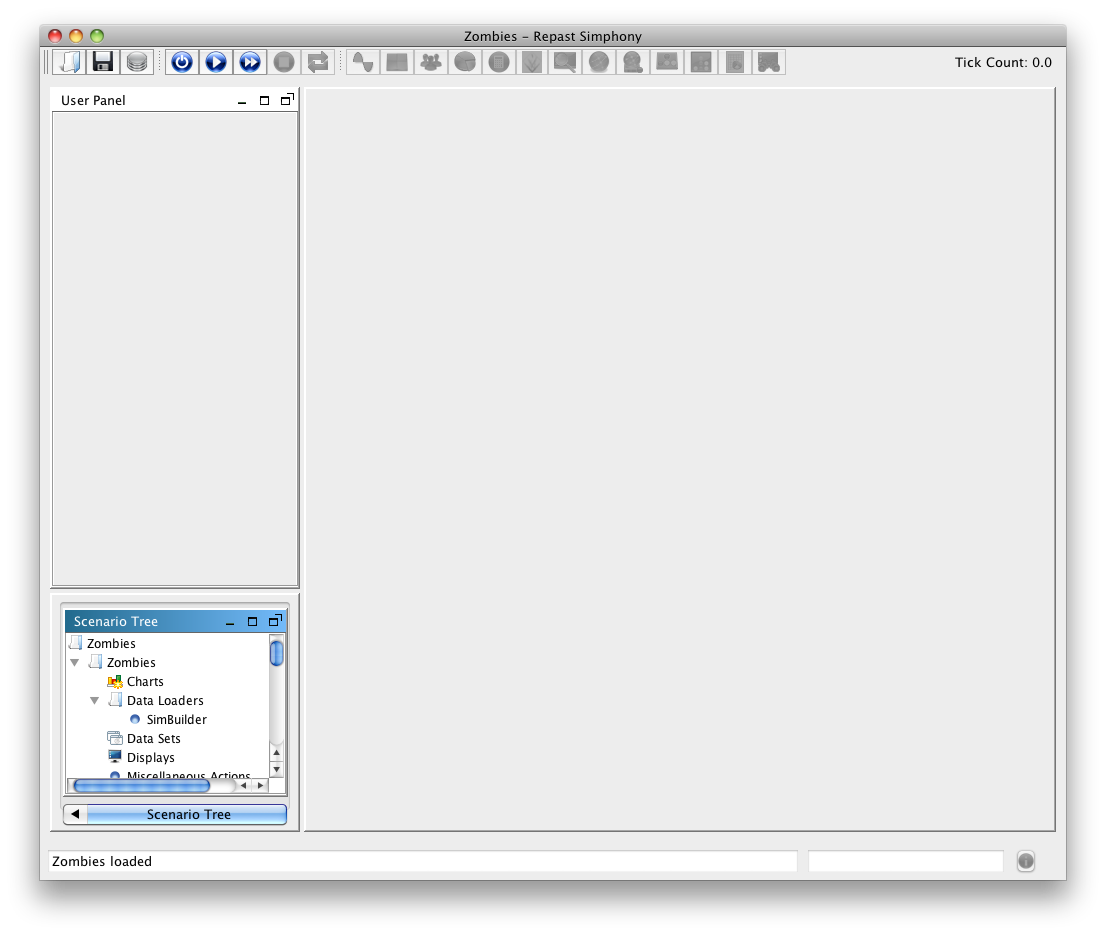
\includegraphics[width=4in]{GettingStartedImages/RepastRuntime.png}
}
\caption{The Repast Simphony runtime.}
\label{fig:repastruntime}
\end{center}
\end{figure}


\begin{figure}
\begin{center}
\vspace{.2in}
\centerline {
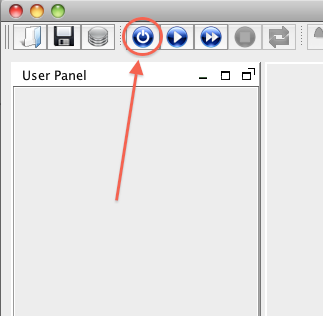
\includegraphics[width=2.5in]{GettingStartedImages/InitializeRuntime.png}
}
\caption{The Initialize button in the Repast Simphony runtime.}
\label{fig:initruntime}
\end{center}
\end{figure}

\begin{figure}
\begin{center}
\vspace{.2in}
\centerline {
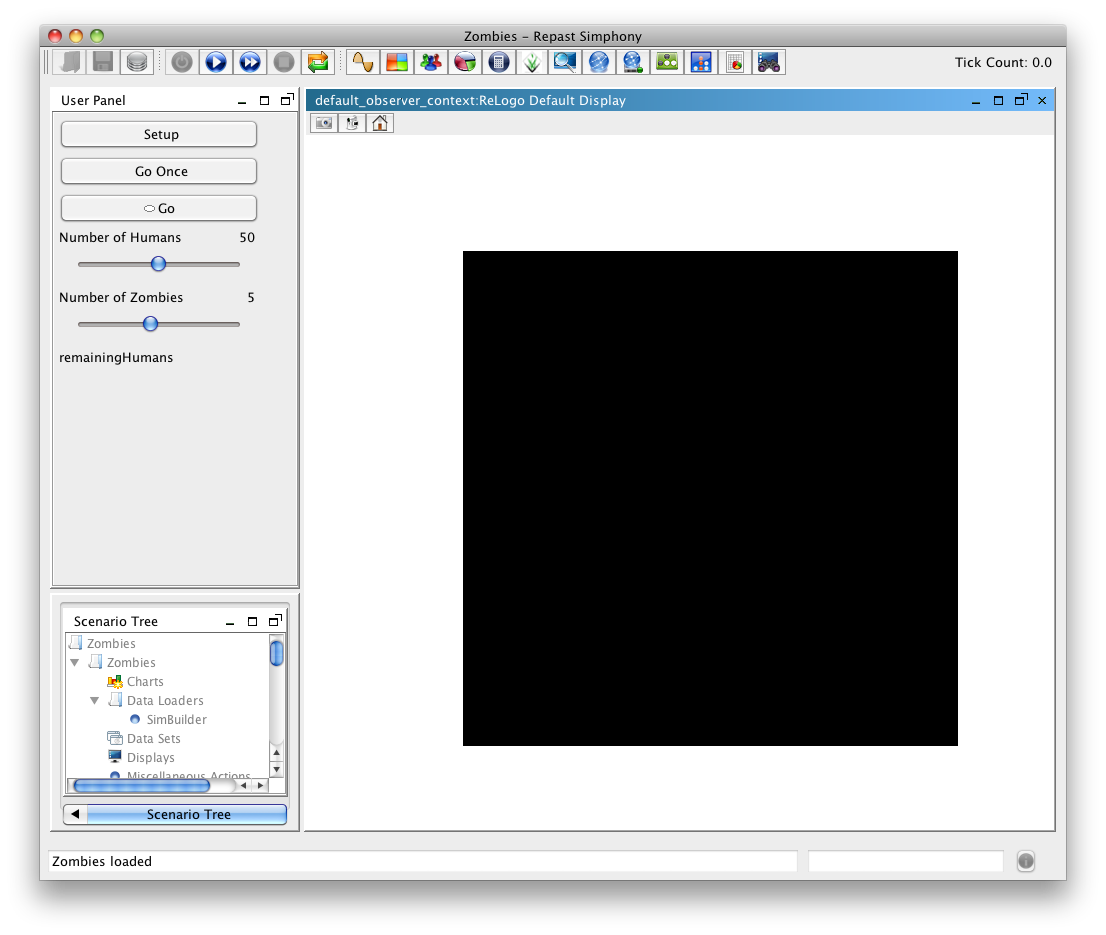
\includegraphics[width=4in]{GettingStartedImages/LoadedZombies.png}
}
\caption{The loaded Zombie model.}
\label{fig:loadedzombies}
\end{center}
\end{figure}

The User Panel on the left reveals the graphical elements that we created (Fig.~\ref{fig:graphelem}). Pressing the Setup button should run the \emph{setup} method we defined earlier in the UserObserver (Listing~\ref{lst:observer2}) which results in Figure~\ref{fig:setupzombies}.

\begin{figure}
\begin{center}
\vspace{.2in}
\centerline {
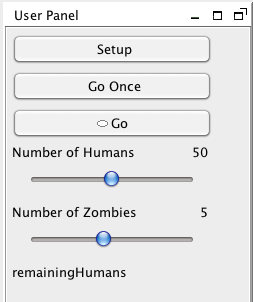
\includegraphics[width=3in]{GettingStartedImages/GraphicalElements.png}
}
\caption{The graphical elements in the User Panel.}
\label{fig:graphelem}
\end{center}
\end{figure}

\begin{figure}
\begin{center}
\vspace{.2in}
\centerline {
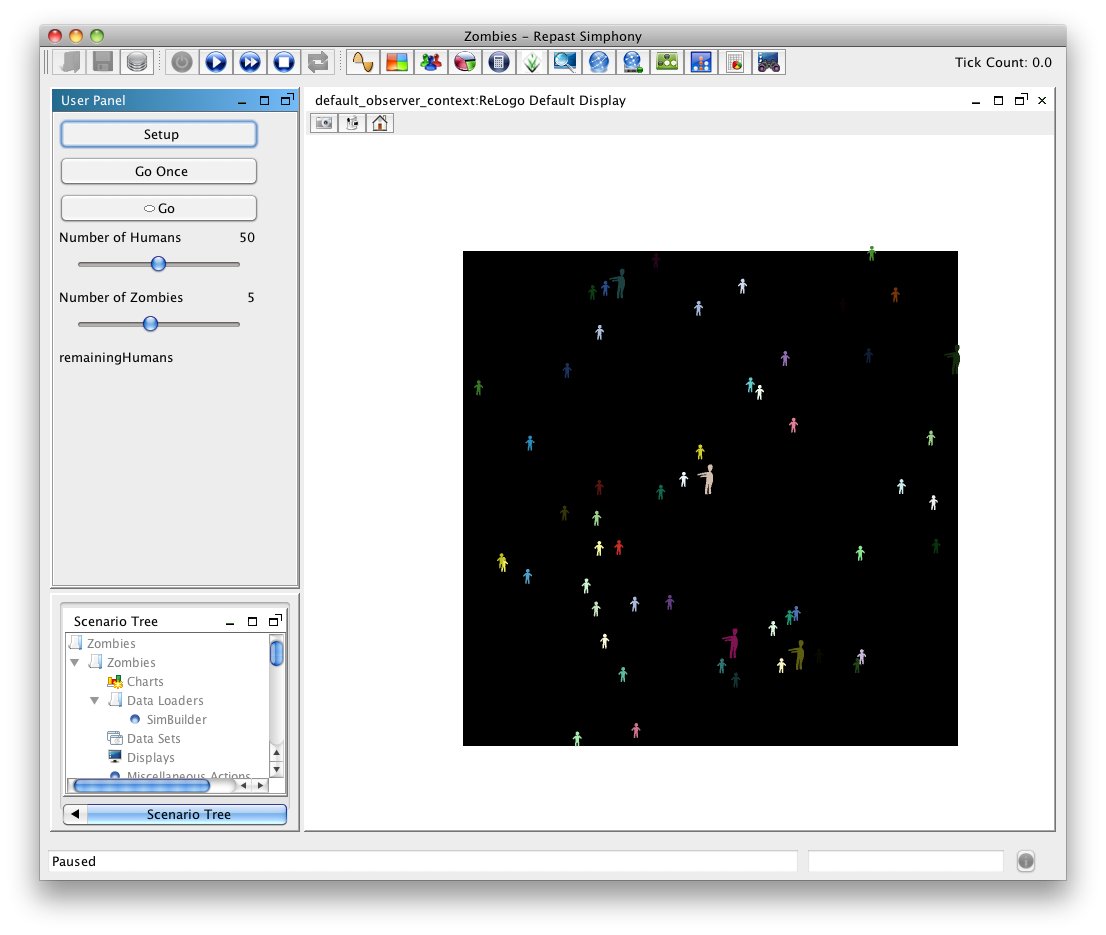
\includegraphics[width=5in]{GettingStartedImages/SetupZombies.png}
}
\caption{The Zombies model after pressing the Setup button.}
\label{fig:setupzombies}
\end{center}
\end{figure}

At this point we can choose to repeatedly press the Go Once button and observe how the model evolves (Fig.~\ref{fig:brains}) or, alternatively, we can press the Go button which will automatically advance the simulation until we un-press it. Whenever we want to reset the model, we simply press the Setup button again.

\begin{figure}
\begin{center}
\vspace{.2in}
\centerline {
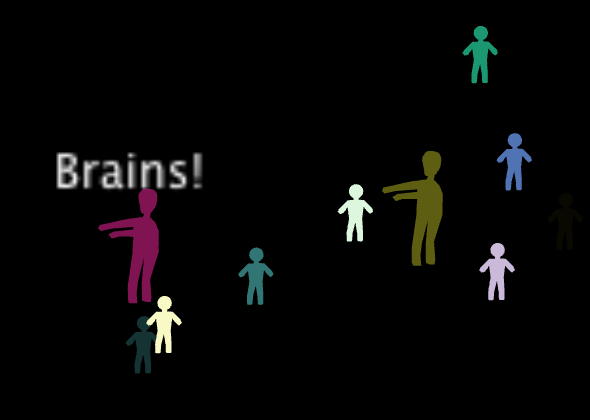
\includegraphics[width=5in]{GettingStartedImages/Brains.png}
}
\caption{A closeup of the Zombies model.}
\label{fig:brains}
\end{center}
\end{figure}

\clearpage
\subsection{Adding links to the Zombies model.}
In this section we'll add to the Zombies model by introducing links\footnote{Links were introduced to Logo by \href{http://ccl.northwestern.edu/netlogo/}{NetLogo}. They are edges of networks where the vertices are the turtles.}. We'll create Infection link types and use them to track which Human agents have been infected by which Zombie agent. We do this, in a similar manner to how we created our Human and Zombie turtle types, by selecting the ``zombies.relogo" package and then clicking on the New Link icon (Fig.~\ref{fig:newlinkicon}) in the toolbar. This brings up the New Link Wizard which allows us to specify the name of our link type. We fill in the Name field with ``Infection" and press the Finish button.

\begin{figure}
\begin{center}
\vspace{.2in}
\centerline {
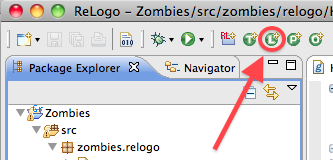
\includegraphics[width=3in]{GettingStartedImages/NewLink.png}
}
\caption{The New Link icon.}
\label{fig:newlinkicon}
\end{center}
\end{figure}

We slightly modify the Zombie \emph{step} method to look like:

\noindent\begin{minipage}[h]{\textwidth}
\vspace{.2in}
\lstset{language=java,caption=New Zombie step method with lines 9~-~11 modified from the previous Zombie step (cf. line 15 in Listing~\ref{lst:zombietype}).,label=lst:newzombiestep}
\begin{lstlisting}
def step(){
	def winner = maxOneOf(neighbors()){
		count(humansOn(it))
	}
	face(winner)
	forward(0.5)
	if (count(humansHere()) > 0){
		label = "Brains!"
		def infectee = oneOf(humansHere()) 
		infect(infectee)
		createInfectionTo(infectee)
	}
	else {
		label = ""
	}
}
\end{lstlisting}
\vspace{.2in}
\end{minipage}
We've made it so that if the Zombie finds a Human, they not only infect the Human but also create an Infection link to it (lines 9~-~11 in Listing~\ref{lst:newzombiestep}). When the infectee dies any links it has are automatically removed so the newly hatched Zombie won't retain those\footnote{It is left to the interested reader to figure out how to make these Infection links persist. There are many possible ways to accomplish this but one is to use the primitives \emph{inInfectionNeighbors} and \emph{createInfectionsFrom}.}. In an analogous manner to how turtle type specific methods were generated when we defined new turtle types, when we create new link types we gain access to a number of new link specific methods. \emph{createInfectionTo} is such a method. To see a full list of the methods generated see Table~\ref{tab:connectionmethods} in Appendix~\ref{app:genprims}.

We'd also like to be able to play with the length of the gestation period, i.e., the period it takes for a Human to die and become a Zombie, to be able to see a network of infections forming before the infected Human dies. We add a gestationPeriod variable as a slider (Listing~\ref{lst:ugpf2}) and modify the Human turtle type (line 17 in Listing~\ref{lst:humantype2}) to accomplish this.

\noindent\begin{minipage}[h]{\textwidth}
\vspace{.2in}
\lstset{language=java,caption=The UserGlobalsAndPanelFactory class with a gestationPeriod variable as a slider.,label=lst:ugpf2}
\begin{lstlisting}
// package declaration and imports, which we can ignore for now

public class UserGlobalsAndPanelFactory
extends AbstractReLogoGlobalsAndPanelFactory{

	public void addGlobalsAndPanelComponents(){
		
		/**
		 * Example comments
		 */
		
		addButtonWL("setup","Setup")
		addButtonWL("go","Go Once")
		addToggleButtonWL("go","Go")
		addSliderWL("numHumans", "Number of Humans", 1, 1, 100, 50)
		addSliderWL("numZombies", "Number of Zombies", 1, 1, 10, 5)
		addSliderWL("gestationPeriod", "Gestation", 5, 1, 30, 5)
		addMonitorWL("remainingHumans", "Remaining Humans", 5)
	}
	
}
\end{lstlisting}
\vspace{.2in}
\end{minipage}

\noindent\begin{minipage}[h]{\textwidth}
\vspace{.2in}
\lstset{language=java,caption=The Human turtle type modified to use a variable gestation period.,label=lst:humantype2}
\begin{lstlisting}
// package declaration and imports, which we can ignore for now

class Human extends BaseTurtle {
	
	def infected = false
	def infectionTime = 0
	
	def step(){
		def winner = minOneOf(neighbors()){
			count(zombiesOn(it))
		}
		face(winner)
		forward(1.5)
		
		if (infected){
			infectionTime++
			if (infectionTime >= gestationPeriod){
				hatchZombies(1){
					size = 2
				}
				die()
			}
		}
	}
	
}
\end{lstlisting}
\vspace{.2in}
\end{minipage}

Now when we run our model, we can see larger networks of Infection links forming as we increase the gestation period (Fig.~\ref{fig:infectionnetworks}).

\begin{figure}
\begin{center}
\vspace{.2in}
\centerline {
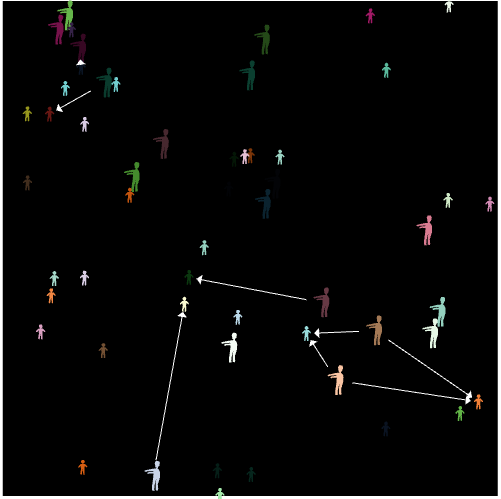
\includegraphics[width=4in]{GettingStartedImages/ZombieNetworks.png}
}
\caption{The Zombie model showing infection networks.}
\label{fig:infectionnetworks}
\end{center}
\end{figure}


\clearpage

\subsection{Data sets, outputters and external plugins.}
Now that we have the model running with turtles, patches and links, we'll explore the creation of simple data sets to create file outputters and even to take advantage of the many plugins available which connect to external tools. We return to our UserObserver class and add the following property and methods:

\noindent\begin{minipage}[h]{\textwidth}
\vspace{.2in}
\lstset{language=java,caption=Additional property and methods in the UserObserver class.,numbers=none}
\begin{lstlisting}
def relogoRun = 0

def remainingZombies(){
	count(zombies())
}

def timestamp(){
	ticks()
}
\end{lstlisting}
\vspace{.2in}
\end{minipage}
The \emph{relogoRun} property will be used to differentiate between runs each time we press the setup button. The \emph{remainingZombies} method is self explanatory. The \emph{timestamp} method returns the current value of the ReLogo counter. This counter is useful for tracking time evolution and a call to \emph{clearAll} re-initializes it. We'll see how to increment this timer below.

In addition, we modify the UserObserver's \emph{setup} and \emph{go} methods in the following ways:

\noindent\begin{minipage}[h]{\textwidth}
\vspace{.2in}
\lstset{language=java,caption=Modified setup and go methods in the UserObserver class.}
\begin{lstlisting}
def setup(){
	relogoRun++
	clearAll()
	setDefaultShape(Human,"person")
	createHumans(numHumans){
		setxy(randomXcor(),randomYcor())
	}
	setDefaultShape(Zombie,"zombie")
	createZombies(numZombies){
		setxy(randomXcor(),randomYcor())
		size = 2
	}
}

def go(){
	ask (zombies()){
		step()
	}
	ask (humans()){
		step()
	}
	tick()
}
\end{lstlisting}
\vspace{.2in}
\end{minipage}
We're incrementing the \emph{relogoRun} property so that we'll be able to differentiate between runs each time \emph{setup} is executed. The \emph{tick} primitive at the end of the \emph{go} method increments the ReLogo counter every time \emph{go} is executed.

The resulting full UserObserver class should now look like:

\noindent\begin{minipage}[h]{\textwidth}
\vspace{.2in}
\lstset{language=java,caption=The full UserObserver class after data set related modifications.}
\begin{lstlisting}
class UserObserver extends BaseObserver{
	def relogoRun = 0
	
	def setup(){
		relogoRun++
		clearAll()
		setDefaultShape(Human,"person")
		createHumans(numHumans){
			setxy(randomXcor(),randomYcor())
		}
		setDefaultShape(Zombie,"zombie")
		createZombies(numZombies){
			setxy(randomXcor(),randomYcor())
			size = 2
		}
	}
	
	def go(){
		ask (zombies()){
			step()
		}
		ask (humans()){
			step()
		}
		tick()
	}
	
	def remainingHumans(){
		count(humans())
	}
	
	def remainingZombies(){
		count(zombies())
	}
	
	def timestamp(){
		ticks()
	}

}
\end{lstlisting}
\vspace{.2in}
\end{minipage}

The next step is to launch the Zombies model. Once it is launched, we go to the Scenario Tree panel underneath the User Panel and carry out the following steps:
\begin{enumerate}
\item
Right click on the Data Sets label (Fig.~\ref{fig:datasetscenario}) and choose Add DataSet.
\item
In the Data Set Editor, type Agent Counts as the Data Set ID, and Non-Aggregate\footnote{The current example is for defining non-aggregate data sources. For an example showing how to create aggregate data sources see the Data Collection section of the \href{http://repast.sourceforge.net/docs/RepastJavaGettingStarted.pdf}{Repast Java Getting Started document}.} as the Data Set type. Click Next.
\item
In the next few steps, we specify the data sources that make up our data set. The Standard Sources tab allows us to add some standard data sources to our data set. For this tutorial we uncheck all of the boxes.
\item
Next, select the Method Data Sources tab. The Method Data Sources tab allows us to create data sources that will call methods on agents in our model. For the Source Class select UserObserver. Click Add to add an entry . Double click in the Method column of the added entry and choose \emph{timestamp} from the drop down list.
\item\label{it:toRepeat}
Click Add again. This time choose \emph{getRelogoRun}\footnote{Groovy automatically generates ``getters" and ``setters" for properties you define. If the property is ``relogoRun" like in this example, the methods \emph{getRelogoRun} and \emph{setRelogoRun} are generated. This capitalization scheme, where the beginning of multiple contiguous words are capitalized, is a standard in many programming languages, including Groovy, and is referred to as ``camel-casing". } from the drop down list.
\item
Repeat Step \ref{it:toRepeat}, but choose \emph{remainingHumans} from the list.
\item
Repeat Step \ref{it:toRepeat}, but choose \emph{remainingZombies} from the drop down list.
\end{enumerate}
\begin{figure}
\begin{center}
\vspace{.2in}
\centerline {
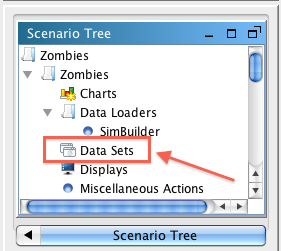
\includegraphics[width=3in]{GettingStartedImages/DataSetScenario.png}
}
\caption{The Data Set label in the Scenario Tree panel.}
\label{fig:datasetscenario}
\end{center}
\end{figure}

At this point you should see the Data Set Editor window looking like Fig.~\ref{fig:datasetcolumns}. Click on Next, then on Finish. Don't forget to save this setting by clicking on the save icon in the top left hand side of the Repast Simphony runtime (Fig.~\ref{fig:save}). Alternatively select Save under the File menu.

\begin{figure}
\begin{center}
\vspace{.2in}
\centerline {
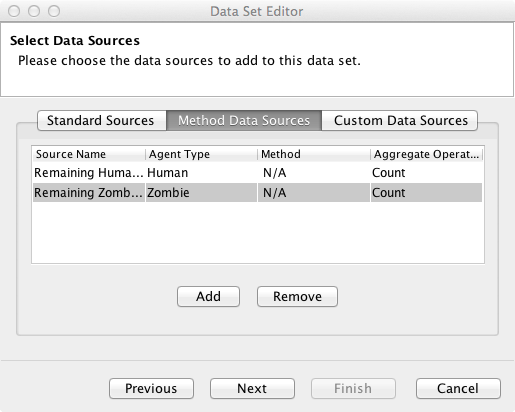
\includegraphics[width=4in]{GettingStartedImages/DataSetColumns.png}
}
\caption{The Data Set Editor window.}
\label{fig:datasetcolumns}
\end{center}
\end{figure}

\begin{figure}
\begin{center}
\vspace{.2in}
\centerline {
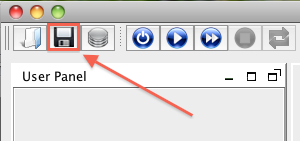
\includegraphics[width=3in]{GettingStartedImages/Save.png}
}
\caption{The Save icon in the Repast Simphony runtime toolbar.}
\label{fig:save}
\end{center}
\end{figure}

Now that we've created a data set we want to be able to output this data set. We have the option of outputting the data set to the console or, as we'll be doing next, to output the data to a file sink. To do this we carry out the following steps:

\begin{enumerate}
\item
Right click on Text Sinks in the Scenario Tree (you may have to scroll down a bit), and click Add File Sink.
\item
Choose Agent Counts for the Data Set ID.
\item
Click on \emph{timestamp} in the first column and click the green right arrow.
\item
Repeat for the remaining items in the column.
\item
Click Next, then Finish (the default location for the text sink is good for the purpose of this guide).
\end{enumerate}
We've chosen the data items from our data set that we wish to output, in this case in comma-delimited form. As we did for the data set, don't forget to save this setting (Fig.~\ref{fig:save}).

Now we initialize the runtime (Fig.~\ref{fig:initruntime}) and run the model via the setup and go buttons. At this point if we quit out of the runtime and return to our workspace we may notice that nothing has changed. However if we select our Zombies project and ``Refresh" it\footnote{The Refresh is necessary when outside processes, in this case our running model, change files from outside the workspace.}, either by right clicking on the project and choosing Refresh from the drop down menu or by pressing the F5 button, we should see the newly generated data file (Fig.~\ref{fig:dataout}). Double-clicking on this file will reveal a comma-delimited four column data set.

\begin{figure}
\begin{center}
\vspace{.2in}
\centerline {
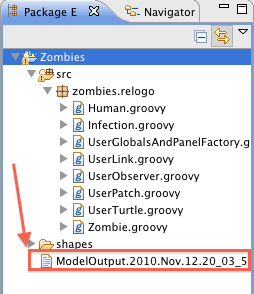
\includegraphics[width=3in]{GettingStartedImages/DataOut.png}
}
\caption{The outputted data in the Zombies model.}
\label{fig:dataout}
\end{center}
\end{figure}

We can also directly connect to some external tools. To demonstrate this, we launch the Zombies model again. After initializing the runtime, and running the model, we turn our attention to the External Tools buttons at the top of the runtime window (Fig.~\ref{fig:externaltools}). For now we'll demonstrate how we can easily export our data into Microsoft Excel. To do this we choose the Spreadsheets plugin, the button with the calculator icon. If you have Excel on your machine, chances are the default location is correct. Otherwise select the appropriate location via the Browse button. Click Next and you should see that the file sink we defined is selected (Fig.~\ref{fig:spreadsheet}). Click Finish and Excel should launch with the data displayed in a spreadsheet. We recommend experimenting with the various other external tool plugins on your own.

\begin{figure}
\begin{center}
\vspace{.2in}
\centerline {
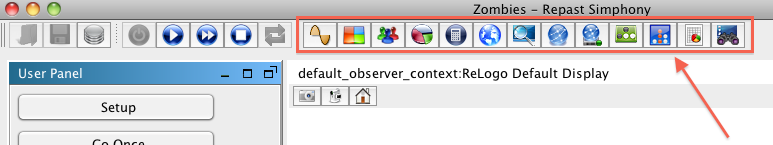
\includegraphics[width=5in]{GettingStartedImages/ExternalTools.png}
}
\caption{The External Tools buttons in the Repast Simphony runtime.}
\label{fig:externaltools}
\end{center}
\end{figure}

\begin{figure}
\begin{center}
\vspace{.2in}
\centerline {
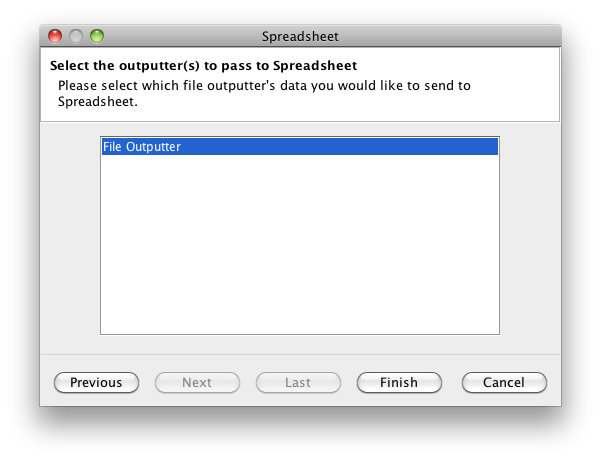
\includegraphics[width=4in]{GettingStartedImages/Spreadsheet.png}
}
\caption{The Spreadsheet wizard with the file sink selected.}
\label{fig:spreadsheet}
\end{center}
\end{figure}






\clearpage

\section{A little more ReLogo.}
We've gone through many of the basics for building models in ReLogo. While there are many more details that are beyond the scope of this getting started guide, below we include a few important items that we haven't covered yet.

\subsection{@Diffusible variables in patches}
Patches can have variables with the @Diffusible annotation:

\noindent\begin{minipage}[h]{\textwidth}
\vspace{.2in}
\lstset{language=java, numbers=none}
\begin{lstlisting}
@Diffusible
def aPatchVariable
\end{lstlisting}
\vspace{.2in}
\end{minipage}

Patch variables annotated this way can be manipulated over all the patches simultaneously with the observer primitives:
\begin{itemize}
\item diffuse(String, double)
\item diffuse4(String, double)
\item diffusibleAdd(String, Number)
\item diffusibleApply(String, DoubleFunction)
\item diffusibleDivide(String, Number)
\item diffusibleMultiply(String, Number)
\item diffusibleSubtract(String, Number)
\end{itemize}

\subsection{@Plural annotation for turtles and links}
The default plural form for turtle and link types is an `s' appended to the class name. Turtle and link types with unusual plural forms can have @Plural annotations specifying custom pluralizations.

\noindent\begin{minipage}[h]{\textwidth}
\vspace{.2in}
\lstset{language=java, numbers=none}
\begin{lstlisting}
@Plural("Mice")
class Mouse extends BaseTurtle {
...
}
\end{lstlisting}
\vspace{.2in}
\end{minipage}
This affects the names of the generated methods in Table~\ref{tab:zombiemethods} and Table~\ref{tab:connectionmethods}. The custom plural forms replace the simple plural forms.


\subsection{@Undirected/@Directed annotations for links}
By default link types are directed. To specify that a link type is undirected, or even to be explicit about a link type being directed, we can use the @Undirected and @Directed annotations on a link class.

\noindent\begin{minipage}[h]{\textwidth}
\vspace{.2in}
\lstset{language=java, numbers=none}
\begin{lstlisting}
@Undirected
class Infection extends BaseLink {
...
}
\end{lstlisting}
\vspace{.2in}
\end{minipage}

\subsection{ReLogo Resource Filter}
\label{sec:RRF}
The default ReLogo workspace's Package Explorer has a ReLogo Resource Filter selected. This hides many of the non-immediately-essential elements in a user project. At some point, however, it will be necessary to deselect this filter to access some of the hidden resources. To do this, select the Package Explorer's view options down arrow (Fig.~\ref{fig:downarrow}) and deselect the ReLogo Resource Filter (Fig.~\ref{fig:resourcefilter})\footnote{If the ReLogo Resource Filter is not visible in the drop down menu, go to the Filters... menu option and there will be an option to deselect it there.}. This will reveal the previously hidden resources. The same procedure applies for reselecting the filter as well.

\begin{figure}
\begin{center}
\vspace{.2in}
\centerline {
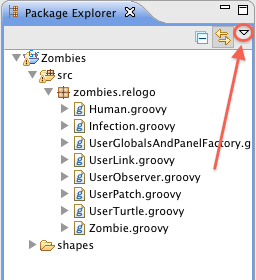
\includegraphics[width=3in]{GettingStartedImages/PackageExplorerArrow.png}
}
\caption{The Package Explorer's view options down arrow.}
\label{fig:downarrow}
\end{center}
\end{figure}

\begin{figure}
\begin{center}
\vspace{.2in}
\centerline {
\includegraphics[width=4in]{GettingStartedImages/PackageExplorerFIlter.png}
}
\caption{The drop down menu for the Package Explorer.}
\label{fig:resourcefilter}
\end{center}
\end{figure}

\subsection{ReLogo world dimensions}
After disabling the ReLogo Resource Filter (Section~\ref{sec:RRF}), one of the elements that can be accessed is the parameters.xml file within the Zombies.rs folder. This is where the world dimensions are stored\footnote{Other parameters can be defined here as well. See the Repast Simphony documentation for details on creating and using custom parameters in your model.}. Double-clicking the file will display the contents in an XML editor (Fig.~\ref{fig:worlddims}) where they can be modified. Note that the dimensions are integers and  ``minPxcor" and  ``minPycor" should be less than or equal to~0.

\begin{figure}
\begin{center}
\vspace{.2in}
\centerline {
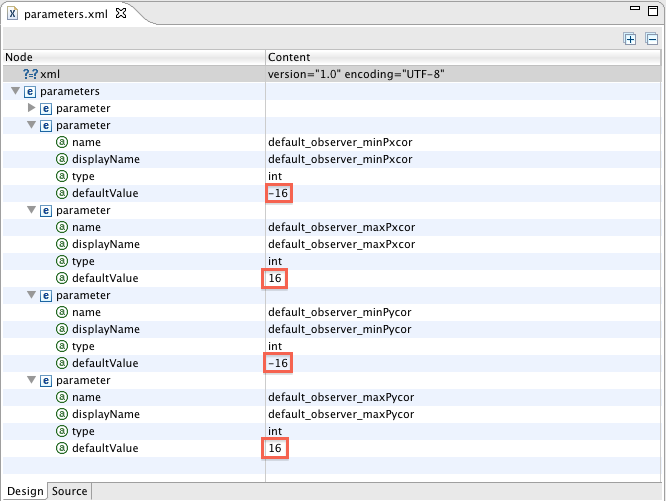
\includegraphics[width=4in]{GettingStartedImages/WorldDimensions.png}
}
\caption{The parameters.xml file with ReLogo world dimensions highlighted.}
\label{fig:worlddims}
\end{center}
\end{figure}

\clearpage
\subsection{Autobuilding}
\label{sec:auto}
A ReLogo model is built when it is launched so by default autobuilding is disabled when a new ReLogo project is created. However, in the case that your workspace has autobuilding enabled and a ReLogo project is imported into the workspace, we recommend that you disable autobuilding yourself, as it won't be disabled automatically. To do this, go to the Project menu and deselect Build Automatically.

\subsection{Default/Recommended Workspace Settings for ReLogo}
\label{sec:defworkspace}
Repast Simphony is distributed with a default workspace. If you have modified your workspace or need to use a custom workspace, the following steps will generate the optimal default workspace settings for ReLogo. 
\begin{itemize}
\item Go to the Preferences menu option (e.g., under the Eclipse menu on Mac OS X, under the Window menu on Windows)
\begin{itemize}
\item Under General $\rightarrow$ Editors $\rightarrow$ Text Editors:
	\begin{itemize}
	\item	Check: Show line numbers
	\end{itemize}
\item Under Groovy:
	\begin{itemize}
	\item Check: Use monospace font for JUnit
	\item Uncheck: Underline staticly unknown references
	\item Uncheck: Do not use parens around methods with arguments
	\item Uncheck: Use brackets for closure arguments
	\end{itemize}
	
\item Under Run/Debug $\rightarrow$ Launching:
	\begin{itemize}
	\item Check:  Always launch the previously launched application
	\end{itemize}
\end{itemize}

\item Select the ReLogo Resource Filter (see~\ref{sec:RRF}):
	
\item Disable Auto Building (see~\ref{sec:auto})

\end{itemize}



%\section{More Advanced Topics}
%Needs work.
%\subsection{Modifying the Default Turtle}
%Needs work.
%By default, commands that refer to �turtle� in a generic way use the UserTurtle turtle type. If, however, you would like to have the generic �turtle� refer to your own custom turtle type, go through the following steps:
%
%\textbf{Need to include mention of disabling ReLogo filter in package explorer.}

\clearpage
\section{Parameter Sweeps and Model Distribution in Repast Simphony}

\subsection{Stochastic Execution and Parameter Sweeps}

Most Repast models use random draws and are therefore stochastic simulations. Stochastic simulations will produce different outcomes for different random number streams, which are generally driven by choosing different random seeds. Such simulations should be executed repeatedly to explore the space of possible outcomes. Even without randomness, model sensitivity analysis parameter sweeps should be run to determine the response of the model to changes in input values. Repast provides both local and distributed tools for automatically completing stochastic execution runs and parameter sweeps. Please see the Repast Parameter Sweep Guide for more information.

\subsection{Model Distribution}

Repast models can be distributed to model users via the installation builder. This feature packs up your model and all of the software you need to run it, except for a properly configured Java Runtime Environment, into a single Java archive ("JAR") file that can be given to model users. The resulting installer can be executed on any system with Java version 1.6 or later; JOGL; and Java3D installed\footnote{Users can obtain free JOGL and Java3D files from the Repast website downloads page \href{http://repast.sourceforge.net/downloads.html}{here}.}. Users simply copy the installer file onto their Windows, Mac OS, or Linux computers and the start the installer by double clicking on the file. Once the installer is started it will show an installation wizard that will prompt the user for the information needed to install the model. If desired, the installer can also be run in a command line mode.

Building an installer for a model is straightforward. Simply choose the ``Build Installer for $\langle$Your Model Name Here$\rangle$ Model" and provide a location and name for the installer file. The installer file's default name is ``setup.jar," which is suitable for most purposes. The install builder will then package and compress your model and the supporting Repast software. The resulting installer files are about 70 MB plus the size of the model code and data. 75 MB to 80 MB is a common total size. 

The Repast install builder uses the IzPack system (http://izpack.org/). More information on installer customization and use, including command line activation, can be found on the \href{http://izpack.org/}{IzPack web site}.

\clearpage
\appendix

\section{Generated ReLogo Primitives}
\label{app:genprims}
When a new turtle type is defined a number of methods become available to turtles, patches, links and observers. The specific methods generated when a Zombie turtle type is defined are listed in Table \ref{tab:zombiemethods}. These are similar in functionality to existing ReLogo primitives with similar names but specialized for the particular turtle type.

\begin{table}[htbp]
   \centering
   \topcaption{Methods generated when a Zombie turtle type is defined.} % requires the topcapt package
   \begin{tabular}{llll } % Column formatting, @{} suppresses leading/trailing space
      \toprule
      \multicolumn{4}{c}{Generated for each} \\
      \midrule
%      \cmidrule(lr){2-3} % Partial rule. (r) trims the line a little bit on the right; (l) & (lr) also possible
           turtle    & patch & link & observer \\
      \midrule
      hatchZombies  & sproutZombies \\
      zombiesHere & zombiesHere \\
      zombiesAt & zombiesAt \\
      zombiesOn & zombiesOn & zombiesOn & zombiesOn \\
      isZombieQ & isZombieQ & isZombieQ & isZombieQ \\
      zombies & zombies & zombies & zombies \\
      zombie & zombie & zombie & zombie \\
      &&& createZombies \\
      &&& createOrderedZombies \\     
     
      \bottomrule
   \end{tabular}
   \label{tab:zombiemethods}
\end{table}

When a new link type is defined methods are generated and become available to turtles, patches, links and observers. The specific methods created when a Connection link type are listed in Table \ref{tab:connectionmethods}. Note that there are differences depending on whether Connection is a directed or undirected link type. Again, these are similar in functionality to existing ReLogo primitives with similar names but specialized for the particular link type.


\begin{table}[htbp]
\begin{minipage}{\linewidth}
   \centering
   \topcaption{Methods generated when a Connection link type is defined.} % requires the topcapt package
   \begin{tabular}{llll } % Column formatting, @{} suppresses leading/trailing space
      \toprule
      \multicolumn{4}{c}{Generated for each\footnote{For a directed link Connection.\label{fn:dir}} \footnote{For an undirected link Connection.\label{fn:und}}}\\
      \midrule
%      \cmidrule(lr){2-3} % Partial rule. (r) trims the line a little bit on the right; (l) & (lr) also possible
           turtle    & patch & link & observer \\
      \midrule
      isConnectionQ & isConnectionQ & isConnectionQ & isConnectionQ \\
      connections & connections & connections & connections \\
      connection & connection & connection & connection \\     
      createConnectionFrom\footref{fn:dir} \\
      createConnectionsFrom\footref{fn:dir} \\
      createConnectionTo\footref{fn:dir} \\
      createConnectionsTo\footref{fn:dir} \\
      createConnectionWith\footref{fn:und} \\
      createConnectionsWith\footref{fn:und} \\
      inConnectionNeighborQ\footref{fn:dir} \\
      inConnectionNeighbors\footref{fn:dir} \\      
      inConnectionFrom\footref{fn:dir} \\
      myInConnections\footref{fn:dir} \\
      myOutConnections\footref{fn:dir} \\
      outConnectionNeighborQ\footref{fn:dir} \\
      outConnectionNeighbors\footref{fn:dir} \\
      outConnectionTo\footref{fn:dir} \\
      connectionNeighborQ \\
      connectionNeighbors \\
      connectionWith\footref{fn:und} \\
      myConnections \\
      \bottomrule
   \end{tabular}

   \label{tab:connectionmethods}
   \end{minipage}
\end{table}


\clearpage
\section{Available Graphical Elements}
\label{app:graphical}

Table \ref{tab:graphical} lists the various elements available for use in the UserGlobalsAndPanelFactory's \emph{addGlobalsAndPanelComponents} method.

% Requires the booktabs if the memoir class is not being used
\begin{table}[htbp]
\begin{minipage}{\linewidth}
   \centering
   \topcaption{Elements available for use in the UserGlobalsAndPanelFactory's \emph{addGlobalsAndPanelComponents} method} % requires the topcapt package
   \begin{tabular}{ ll } % Column formatting, @{} suppresses leading/trailing space
      \toprule
           Element Types    & Commands\footnote{The (WL) refers to variants \emph{with labels}.} \\
      \midrule
      Button      & addButton(WL)\footnote{Include variants with observer specified by id.\label{fn:obs}}\\
      State Change Button\footnote{State change buttons do not advance the simulation schedule.} & addStateChangeButton(WL)\footref{fn:obs} \\
     ToggleButton & addToggleButton(WL)\footref{fn:obs} \\
     Slider & addSlider(WL) \\
     Chooser & addChooser(WL) \\
     Switch & addSwitch(WL) \\
     Input & addInput \\
     Monitor & addMonitor \\
     Global & addGlobal \\
     
      \bottomrule
   \end{tabular}
   \label{tab:graphical}
      \end{minipage}
\end{table}
Additionally, \emph{Observer}s are provided with a \emph{registerModelParameterListener(String,Closure)} method which allows for registering a closure to execute when a specified model parameter (such as those defined by the Global, Slider, Chooser, Switch and Input elements) are modified. This method would typically be called from within a \emph{setup}-like \emph{Observer} method.

Groovy's \href{http://groovy.codehaus.org/Swing+Builder}{SwingBuilder} can also be used to create more advanced GUIs. The elements available are listed in Table \ref{tab:graphical2}. Listing \ref{lst:swingbuilder} shows a code snippet example. Note that the usage pattern of the elements in Table~\ref{tab:graphical2} is to assign the elements to a variable and use SwingBuilder's \emph{widget} method to incorporate them into panels you create with \emph{addPanel}\footnote{The \emph{addPanel} method passes its closure argument to a SwingBuilder \emph{panel} element.}.

% Requires the booktabs if the memoir class is not being used
\begin{table}[htbp]
\begin{minipage}{\linewidth}
   \centering
   \topcaption{Elements available for use with Groovy's SwingBuilder in the UserGlobalsAndPanelFactory's \emph{addGlobalsAndPanelComponents} method} % requires the topcapt package
   \begin{tabular}{ ll } % Column formatting, @{} suppresses leading/trailing space
      \toprule
           Element Types    & Commands\footnote{The (WL) refers to variants \emph{with labels}.} \\
      \midrule
      Panel  & addPanel \\
      Button      & button(WL)\footnote{Include variants with observer specified by id.\label{fn:obs2}}\\
     ToggleButton & toggleButton(WL)\footref{fn:obs2} \\
     Slider & slider(WL) \\
     Chooser & chooser(WL) \\
     Switch & rSwitch(WL) \\
     Input & input \\
     Monitor & monitor \\
     
      \bottomrule
   \end{tabular}
   \label{tab:graphical2}
      \end{minipage}
\end{table}

\noindent\begin{minipage}[h]{\textwidth}
\vspace{.2in}
\lstset{language=java,caption=Using Groovy's SwingBuilder for building GUIs.,label=lst:swingbuilder}
\begin{lstlisting}
def setupB = buttonWL("setup","Set up the Sim")
def goTB = toggleButtonWL("go","Continuous Go")
addPanel{
	gridLayout(columns:1, rows:0)
	widget(setupB)
	widget(goTB)
}
\end{lstlisting}
\vspace{.2in}
\end{minipage}

\clearpage
\section{More on Turtle Shapes}
\label{app:drawing}
Any image file that's placed in the shapes folder of a ReLogo project can be referred to by name (minus suffix) within the model. Different platforms will have some minor differences in the types of image files that are readable but most of the standard ones can be used (e.g., ``jpeg", ``pbm", ``bmp", ``jpg", ``wbmp", ``ppm", ``png", ``jp2", ``pgm", ``gif"). In addition to regular image files, ReLogo allows one to create svg files that can either be used as images, which we refer to as ``complex'' svg files, or as shapes which have specified regions with fixed colors and regions whose colors can be changed within a ReLogo simulation. The default svg files that come with any newly created ReLogo project are of the latter type, which we refer to as ``simple'' svg files.

We recommend the free and open source SVG editor \href{http://inkscape.org/}{Inkscape} for creating svg images. There are some keywords that can be used to define the special ReLogo properties of an svg file you create. These are specified as a comma delimited list in the ``Keywords'' field of the file's Document Metadata (File $\rightarrow$ Document Metadata...):
\begin{itemize}
  \item simple: indicates that the svg file is simple (assumed complex if not specified)
  \item rotate: indicates whether the icon should rotate according to the turtle's heading 
  \item offset \emph{value}: indicates the clockwise offset (in degrees) of the shape
\end{itemize}

To fix the color of an element within a simple svg file right click on the element and select ``Object Properties.'' In the Description field enter ``fixedColor'' and the element will retain its color. All other elements in a simple svg will take on the color assigned to the turtle within a simulation.

\end{document}  